% Options for packages loaded elsewhere
\PassOptionsToPackage{unicode}{hyperref}
\PassOptionsToPackage{hyphens}{url}
%
\documentclass[
  11pt,
  a4paper,
]{article}
\usepackage{amsmath,amssymb}
\usepackage{lmodern}
\usepackage{iftex}
\ifPDFTeX
  \usepackage[T1]{fontenc}
  \usepackage[utf8]{inputenc}
  \usepackage{textcomp} % provide euro and other symbols
\else % if luatex or xetex
  \ifXeTeX
    \usepackage{zxjatype} 
    \usepackage[ipaex]{zxjafont}
    \setromanfont{Times New Roman}
  \fi
  \usepackage{unicode-math}
  \defaultfontfeatures{Scale=MatchLowercase}
  \defaultfontfeatures[\rmfamily]{Ligatures=TeX,Scale=1}
\fi
% Use upquote if available, for straight quotes in verbatim environments
\IfFileExists{upquote.sty}{\usepackage{upquote}}{}
\IfFileExists{microtype.sty}{% use microtype if available
  \usepackage[]{microtype}
  \UseMicrotypeSet[protrusion]{basicmath} % disable protrusion for tt fonts
}{}
\usepackage{xcolor}
\IfFileExists{xurl.sty}{\usepackage{xurl}}{} % add URL line breaks if available
\IfFileExists{bookmark.sty}{\usepackage{bookmark}}{\usepackage{hyperref}}
\hypersetup{
  pdftitle={補論:風しんの抗体検査とワクチン接種を促進するためのナッジ・メッセージの探求},
  hidelinks,
  pdfcreator={LaTeX via pandoc}}
\urlstyle{same} % disable monospaced font for URLs
\usepackage[left=3cm,right=3cm,top=3cm,bottom=3cm]{geometry}

\usepackage{setspace}
\renewcommand{\baselinestretch}{1.5}
\usepackage{float}

\usepackage{longtable,booktabs,array}
\usepackage{threeparttable, threeparttablex, multirow}
\usepackage{calc} % for calculating minipage widths
% Correct order of tables after \paragraph or \subparagraph
\usepackage{etoolbox}
\makeatletter
\patchcmd\longtable{\par}{\if@noskipsec\mbox{}\fi\par}{}{}
\makeatother
% Allow footnotes in longtable head/foot
\IfFileExists{footnotehyper.sty}{\usepackage{footnotehyper}}{\usepackage{footnote}}
\makesavenoteenv{longtable}
\renewcommand{\figurename}{図}
\renewcommand{\tablename}{表}
\usepackage{graphicx}
\makeatletter
\def\maxwidth{\ifdim\Gin@nat@width>\linewidth\linewidth\else\Gin@nat@width\fi}
\def\maxheight{\ifdim\Gin@nat@height>\textheight\textheight\else\Gin@nat@height\fi}
\makeatother
% Scale images if necessary, so that they will not overflow the page
% margins by default, and it is still possible to overwrite the defaults
% using explicit options in \includegraphics[width, height, ...]{}
\setkeys{Gin}{width=\maxwidth,height=\maxheight,keepaspectratio}
% Set default figure placement to htbp
\makeatletter
\def\fps@figure{htbp}
\makeatother
\setlength{\emergencystretch}{3em} % prevent overfull lines
\providecommand{\tightlist}{%
  \setlength{\itemsep}{0pt}\setlength{\parskip}{0pt}}
\setcounter{secnumdepth}{5}


\usepackage{float}
\ifLuaTeX
  \usepackage{selnolig}  % disable illegal ligatures
\fi

\makeatletter
\def\@fnsymbol#1{\ensuremath{\ifcase#1\or \dagger\or \ddagger\or
   \mathsection\or \mathparagraph\or \|\or **\or \dagger\dagger
   \or \ddagger\ddagger \else\@ctrerr\fi}}
    \makeatother
\title{補論:風しんの抗体検査とワクチン接種を促進するためのナッジ・メッセージの探求  }

\date{2022/04/07}



\begin{document}
\begin{spacing}{1}
  \maketitle
\end{spacing}

\hypertarget{appendix-appendix}{%
\appendix}


\hypertarget{additional-tabels-and-figures}{%
\section{Additional Tabels and Figures}\label{additional-tabels-and-figures}}

\begin{figure}[t]
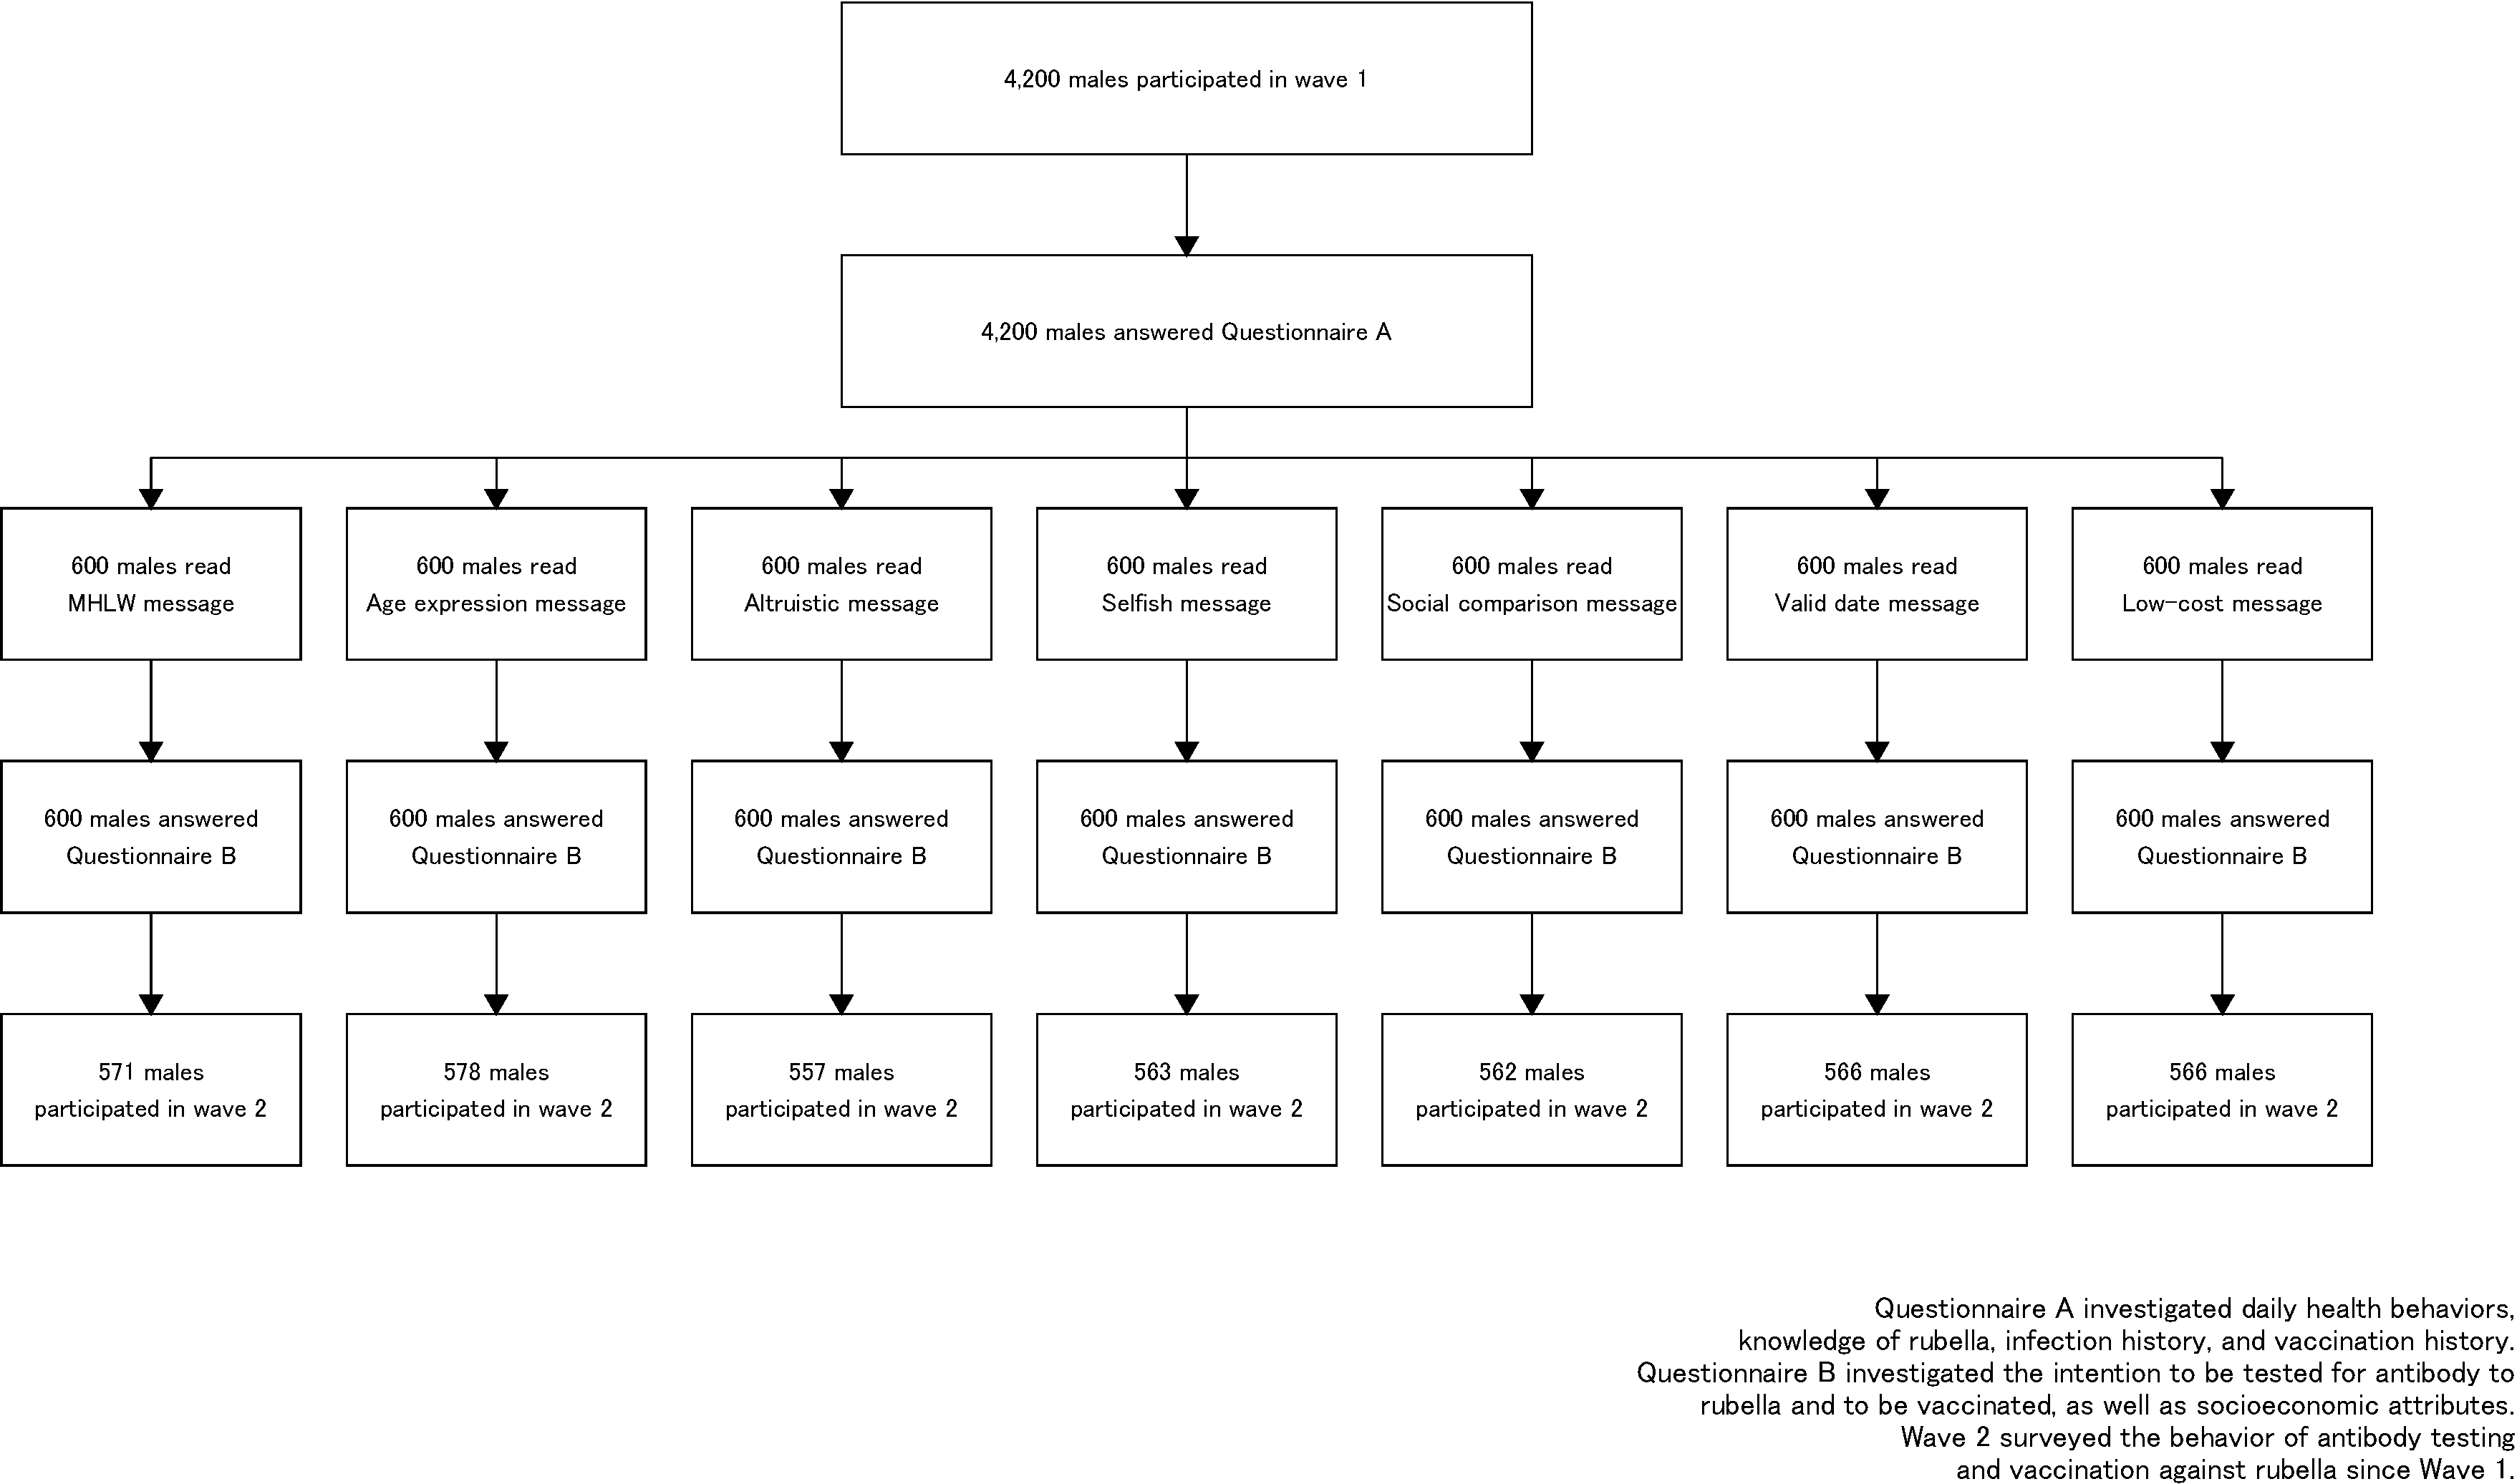
\includegraphics[width=1.5\linewidth,angle=90]{C:/Users/vge00/Desktop/MHLW-Rubella-Project/2020-online-RCT/publish/appendix_files/figure-latex/show-flowchart-1} \caption{オンライン調査の概要}\label{fig:show-flowchart}
\end{figure}

\begin{table}[!h]

\caption{\label{tab:show-covlist}共変量の一覧}
\centering
\fontsize{9}{11}\selectfont
\begin{tabular}[t]{l>{\raggedright\arraybackslash}p{30em}cc}
\toprule
  & 変数の説明 & Mean & Std.Dev.\\
\midrule
age & (Wave1) 生まれ年と生まれつきに基づいて計算した2019年4月時点の年齢 & 48.66 & 5.69\\
coupon2019 & (Wave1) 2019年4月時点で40歳以上46歳以下(2019年度クーポン券配布対象)ならば1を取るダミー変数 & 0.35 & 0.48\\
married & (Wave1) 婚姻したら1を取るダミー変数 & 0.58 & 0.49\\
education & (Wave1) 教育年数 & 14.75 & 2.31\\
exercise\_w1 & (Wave1) 週に1度以上運動やスポーツをしていたら1を取るダミー変数 & 0.22 & 0.42\\
health\_check & (Wave1) 調査時点から過去1年間で職場や自治体の健康診断を受けたら1を取るダミー変数 & 0.68 & 0.46\\
flushot & (Wave1) 毎年インフルエンザワクチンを接種しているならば1を取るダミー変数 & 0.27 & 0.45\\
prob\_social & (Wave1) 40代・50代が風しんに感染する確率はどれくらいか? & 30.38 & 19.87\\
handicap & (Wave1)妊娠初期の女性が風しんに感染したら、障害を持った子供が産まれる可能性があると回答者が信じているならば、1を取るダミー変数 & 0.63 & 0.48\\
severity & (Wave1) 成人男性が風しんに感染すると、重症化する可能性があると回答者が信じているならば、1を取るダミー変数 & 0.92 & 0.27\\
handwash & (Wave2)「前回の調査から今日までの期間で、こまめに手洗い・うがいをしている」という文章に対する5段階評価(1:全く当てはまらない~5:非常に当てはまる) & 3.91 & 1.04\\
temp\_check & (Wave2)「前回の調査から今日までの期間で、こまめに体温を測定している」という文章に対する5段階評価(1:全く当てはまらない~5:非常に当てはまる) & 2.26 & 1.22\\
avoid\_out & (Wave2)「前回の調査から今日までの期間で、外出を控えている」という文章に対する5段階評価(1:全く当てはまらない~7:非常に当てはまる) & 2.96 & 1.20\\
avoid\_crowd & (Wave2)「前回の調査から今日までの期間で、外出するときは、人ごみの多い場所を避けている」という文章に対する5段階評価(1:全く当てはまらない~8:非常に当てはまる) & 3.38 & 1.10\\
wear\_mask & (Wave2)「前回の調査から今日までの期間で、外出するときや人と会うときは、必ずマスクを着用している」という文章に対する5段階評価(1:全く当てはまらない~9:非常に当てはまる) & 3.14 & 1.38\\
\bottomrule
\end{tabular}
\end{table}

\begin{table}

\caption{\label{tab:show-int-coupon1-balance}Wave 1セレクションデータの共変量のバランステスト(2019年度クーポン券配布対象)}
\centering
\begin{tabular}[t]{lcccccccc}
\toprule
\multicolumn{1}{c}{ } & \multicolumn{7}{c}{Treatments} & \multicolumn{1}{c}{ } \\
\cmidrule(l{3pt}r{3pt}){2-8}
  & 厚労省 & 年齢表現 & 利他強調 & 利己強調 & 社会比較 & 有効期限 & 低コスト & p-value\\
\midrule
age & 42.862 & 43.046 & 43.135 & 43.045 & 42.909 & 42.906 & 42.866 & 0.874\\
avoid\_crowd & 3.328 & 3.331 & 3.261 & 3.211 & 3.339 & 3.336 & 3.273 & 0.958\\
avoid\_out & 3.082 & 3.047 & 3.028 & 2.805 & 2.896 & 3.038 & 2.926 & 0.509\\
education & 14.654 & 14.473 & 14.595 & 14.205 & 14.099 & 14.348 & 14.575 & 0.446\\
exercise\_w1 & 0.246 & 0.176 & 0.277 & 0.189 & 0.165 & 0.217 & 0.213 & 0.285\\
flushot & 0.238 & 0.260 & 0.203 & 0.144 & 0.140 & 0.239 & 0.236 & 0.055\\
handicap & 0.638 & 0.550 & 0.595 & 0.568 & 0.537 & 0.543 & 0.520 & 0.502\\
handwash & 3.885 & 3.866 & 3.824 & 3.764 & 3.748 & 3.954 & 3.744 & 0.624\\
health\_check & 0.654 & 0.626 & 0.696 & 0.538 & 0.603 & 0.674 & 0.614 & 0.150\\
married & 0.408 & 0.458 & 0.412 & 0.417 & 0.455 & 0.478 & 0.480 & 0.785\\
prob\_social & 27.231 & 30.000 & 26.689 & 30.758 & 26.529 & 28.333 & 27.795 & 0.502\\
severity & 0.892 & 0.954 & 0.926 & 0.894 & 0.926 & 0.964 & 0.913 & 0.118\\
temp\_check & 2.180 & 2.260 & 2.380 & 2.179 & 2.226 & 2.145 & 2.157 & 0.735\\
wear\_mask & 2.951 & 3.063 & 3.113 & 3.033 & 2.965 & 3.115 & 3.174 & 0.852\\
\bottomrule
\end{tabular}
\end{table}

\begin{table}

\caption{\label{tab:show-act-coupon1-balance}Wave 1セレクションデータの共変量のバランステスト(2019年度クーポン券配布対象)}
\centering
\begin{tabular}[t]{lcccccccc}
\toprule
\multicolumn{1}{c}{ } & \multicolumn{7}{c}{Treatments} & \multicolumn{1}{c}{ } \\
\cmidrule(l{3pt}r{3pt}){2-8}
  & 厚労省 & 年齢表現 & 利他強調 & 利己強調 & 社会比較 & 有効期限 & 低コスト & p-value\\
\midrule
age & 42.861 & 43.059 & 43.102 & 43.036 & 42.893 & 42.898 & 42.964 & 0.953\\
avoid\_crowd & 3.296 & 3.336 & 3.273 & 3.234 & 3.350 & 3.305 & 3.324 & 0.990\\
avoid\_out & 3.096 & 3.034 & 3.047 & 2.793 & 2.932 & 3.025 & 2.928 & 0.544\\
education & 14.496 & 14.471 & 14.547 & 14.126 & 14.010 & 14.407 & 14.595 & 0.474\\
exercise\_w1 & 0.252 & 0.185 & 0.266 & 0.171 & 0.165 & 0.195 & 0.225 & 0.375\\
flushot & 0.235 & 0.261 & 0.227 & 0.135 & 0.146 & 0.246 & 0.207 & 0.082\\
handicap & 0.652 & 0.563 & 0.602 & 0.568 & 0.544 & 0.542 & 0.514 & 0.425\\
handwash & 3.861 & 3.916 & 3.797 & 3.757 & 3.767 & 3.915 & 3.829 & 0.835\\
health\_check & 0.643 & 0.639 & 0.680 & 0.532 & 0.631 & 0.661 & 0.640 & 0.391\\
married & 0.391 & 0.454 & 0.391 & 0.360 & 0.437 & 0.466 & 0.477 & 0.467\\
prob\_social & 27.739 & 30.504 & 27.031 & 31.982 & 26.311 & 28.729 & 28.018 & 0.341\\
severity & 0.896 & 0.950 & 0.922 & 0.883 & 0.913 & 0.975 & 0.910 & 0.026\\
temp\_check & 2.139 & 2.235 & 2.414 & 2.126 & 2.204 & 2.203 & 2.117 & 0.535\\
wear\_mask & 2.930 & 3.076 & 3.109 & 3.009 & 3.010 & 3.144 & 3.207 & 0.794\\
\bottomrule
\end{tabular}
\end{table}

\begin{table}

\caption{\label{tab:show-int-coupon1-reg}2019年度クーポン券配布対象者に限定した 抗体検査とワクチン接種の意向の線形確率モデルの推定結果}
\centering
\begin{threeparttable}
\begin{tabular}[t]{lcccc}
\toprule
\multicolumn{1}{c}{ } & \multicolumn{2}{c}{抗体検査} & \multicolumn{2}{c}{ワクチン接種} \\
\cmidrule(l{3pt}r{3pt}){2-3} \cmidrule(l{3pt}r{3pt}){4-5}
  & (1) & (2) & (3) & (4)\\
\midrule
年齢表現 & 0.021 & 0.013 & 0.020 & 0.006\\
 & (0.051) & (0.051) & (0.061) & (0.061)\\
利他強調 & 0.144*** & 0.151*** & 0.024 & 0.022\\
 & (0.053) & (0.052) & (0.059) & (0.059)\\
利己強調 & 0.073 & 0.091* & 0.039 & 0.048\\
 & (0.053) & (0.052) & (0.061) & (0.061)\\
社会比較 & 0.040 & 0.079 & 0.014 & 0.021\\
 & (0.053) & (0.052) & (0.062) & (0.061)\\
有効期限 & 0.031 & 0.026 & -0.010 & -0.021\\
 & (0.051) & (0.050) & (0.060) & (0.060)\\
低コスト & 0.052 & 0.053 & 0.018 & 0.014\\
 & (0.053) & (0.051) & (0.062) & (0.061)\\
\midrule
Num.Obs. & 927 & 881 & 927 & 881\\
R2 & 0.269 & 0.364 & 0.431 & 0.498\\
R2 Adj. & 0.263 & 0.349 & 0.427 & 0.486\\
共変量 &  & X &  & X\\
\bottomrule
\end{tabular}
\begin{tablenotes}
\item 注)* p < 0.1、** p < 0.05、*** p < 0.01。頑健標準誤差を使用している。 共変量は補論\ref{addtab}の表\ref{tab:covlist}に示した変数をすべて使用している。
\end{tablenotes}
\end{threeparttable}
\end{table}

\begin{table}

\caption{\label{tab:show-act-coupon1-reg}2019年度クーポン券配布対象者に限定した 抗体検査とワクチン接種の行動の線形確率モデルの推定結果}
\centering
\begin{threeparttable}
\begin{tabular}[t]{lcccc}
\toprule
\multicolumn{1}{c}{ } & \multicolumn{2}{c}{抗体検査} & \multicolumn{2}{c}{抗体検査×ワクチン接種} \\
\cmidrule(l{3pt}r{3pt}){2-3} \cmidrule(l{3pt}r{3pt}){4-5}
  & (1) & (2) & (3) & (4)\\
\midrule
年齢表現 & 0.032 & 0.030 & 0.008 & 0.007\\
 & (0.029) & (0.028) & (0.015) & (0.015)\\
利他強調 & 0.075** & 0.073** & 0.038* & 0.037*\\
 & (0.032) & (0.032) & (0.021) & (0.021)\\
利己強調 & 0.055* & 0.067** & 0.018 & 0.022\\
 & (0.032) & (0.032) & (0.018) & (0.018)\\
社会比較 & 0.053 & 0.065** & 0.040* & 0.045*\\
 & (0.033) & (0.033) & (0.023) & (0.023)\\
有効期限 & 0.008 & 0.008 & 0.000 & 0.001\\
 & (0.025) & (0.025) & (0.012) & (0.012)\\
低コスト & 0.037 & 0.041 & 0.018 & 0.022\\
 & (0.030) & (0.029) & (0.018) & (0.018)\\
\midrule
Num.Obs. & 805 & 805 & 805 & 805\\
R2 & 0.081 & 0.106 & 0.035 & 0.061\\
R2 Adj. & 0.073 & 0.082 & 0.027 & 0.036\\
共変量 &  & X &  & X\\
\bottomrule
\end{tabular}
\begin{tablenotes}
\item 注)* p < 0.1、** p < 0.05、*** p < 0.01。頑健標準誤差を使用している。 共変量は補論\ref{addtab}の表\ref{tab:covlist}に示した変数をすべて使用している。
\end{tablenotes}
\end{threeparttable}
\end{table}

\begin{table}

\caption{\label{tab:show-int-coupon1-altreg}利他強調メッセージと比較した意向に対する介入群の効果 (2019年度クーポン券配布対象者)}
\centering
\begin{threeparttable}
\begin{tabular}[t]{lcccc}
\toprule
\multicolumn{1}{c}{ } & \multicolumn{2}{c}{抗体検査} & \multicolumn{2}{c}{ワクチン接種} \\
\cmidrule(l{3pt}r{3pt}){2-3} \cmidrule(l{3pt}r{3pt}){4-5}
  & (1) & (2) & (3) & (4)\\
\midrule
厚労省 & -0.144*** & -0.151*** & -0.024 & -0.022\\
 & (0.053) & (0.052) & (0.059) & (0.059)\\
年齢表現 & -0.122** & -0.138*** & -0.004 & -0.016\\
 & (0.054) & (0.052) & (0.060) & (0.058)\\
利己強調 & -0.071 & -0.061 & 0.015 & 0.026\\
 & (0.055) & (0.054) & (0.060) & (0.058)\\
社会比較 & -0.103* & -0.072 & -0.009 & -0.001\\
 & (0.056) & (0.054) & (0.061) & (0.058)\\
有効期限 & -0.112** & -0.125** & -0.033 & -0.043\\
 & (0.053) & (0.052) & (0.058) & (0.058)\\
低コスト & -0.092* & -0.098* & -0.006 & -0.008\\
 & (0.055) & (0.052) & (0.060) & (0.058)\\
\midrule
Num.Obs. & 927 & 881 & 927 & 881\\
R2 & 0.269 & 0.364 & 0.431 & 0.498\\
R2 Adj. & 0.263 & 0.349 & 0.427 & 0.486\\
共変量 &  & X &  & X\\
\bottomrule
\end{tabular}
\begin{tablenotes}
\item 注)* p < 0.1、** p < 0.05、*** p < 0.01。頑健標準誤差を使用している。 共変量は補論\ref{addtab}の表\ref{tab:covlist}に示した変数をすべて使用している。
\end{tablenotes}
\end{threeparttable}
\end{table}

\begin{table}

\caption{\label{tab:show-act-coupon1-altreg}利他強調メッセージと比較した意向に対する介入群の効果 (2019年度クーポン券配布対象者)}
\centering
\begin{threeparttable}
\begin{tabular}[t]{lcccc}
\toprule
\multicolumn{1}{c}{ } & \multicolumn{2}{c}{抗体検査} & \multicolumn{2}{c}{抗体検査×ワクチン接種} \\
\cmidrule(l{3pt}r{3pt}){2-3} \cmidrule(l{3pt}r{3pt}){4-5}
  & (1) & (2) & (3) & (4)\\
\midrule
厚労省 & -0.075** & -0.073** & -0.038* & -0.037*\\
 & (0.032) & (0.032) & (0.021) & (0.021)\\
年齢表現 & -0.042 & -0.043 & -0.030 & -0.029\\
 & (0.036) & (0.036) & (0.022) & (0.022)\\
利己強調 & -0.019 & -0.006 & -0.020 & -0.014\\
 & (0.039) & (0.038) & (0.024) & (0.023)\\
社会比較 & -0.022 & -0.008 & 0.002 & 0.008\\
 & (0.039) & (0.039) & (0.028) & (0.028)\\
有効期限 & -0.067** & -0.066** & -0.038* & -0.036*\\
 & (0.033) & (0.033) & (0.021) & (0.021)\\
低コスト & -0.037 & -0.032 & -0.020 & -0.014\\
 & (0.037) & (0.036) & (0.024) & (0.024)\\
\midrule
Num.Obs. & 805 & 805 & 805 & 805\\
R2 & 0.081 & 0.106 & 0.035 & 0.061\\
R2 Adj. & 0.073 & 0.082 & 0.027 & 0.036\\
共変量 &  & X &  & X\\
\bottomrule
\end{tabular}
\begin{tablenotes}
\item 注)* p < 0.1、** p < 0.05、*** p < 0.01。頑健標準誤差を使用している。 共変量は補論\ref{addtab}の表\ref{tab:covlist}に示した変数をすべて使用している。
\end{tablenotes}
\end{threeparttable}
\end{table}

\hypertarget{econvalue}{%
\subsection{ナッジ・メッセージの金銭的価値}\label{econvalue}}

\begin{table}

\caption{\label{tab:show-int-coupon0-balance}Wave 1セレクションデータの共変量のバランステスト(2019年度クーポン券配布対外)}
\centering
\begin{tabular}[t]{lcccccccc}
\toprule
\multicolumn{1}{c}{ } & \multicolumn{7}{c}{Treatments} & \multicolumn{1}{c}{ } \\
\cmidrule(l{3pt}r{3pt}){2-8}
  & 厚労省 & 年齢表現 & 利他強調 & 利己強調 & 社会比較 & 有効期限 & 低コスト & p-value\\
\midrule
age & 51.632 & 51.408 & 51.226 & 51.657 & 51.582 & 51.545 & 51.502 & 0.712\\
avoid\_crowd & 3.307 & 3.378 & 3.429 & 3.250 & 3.306 & 3.296 & 3.455 & 0.354\\
avoid\_out & 2.903 & 2.917 & 2.919 & 2.884 & 2.825 & 2.966 & 2.982 & 0.848\\
education & 14.572 & 14.655 & 14.530 & 14.830 & 14.566 & 14.634 & 14.393 & 0.578\\
exercise\_w1 & 0.156 & 0.193 & 0.239 & 0.230 & 0.183 & 0.203 & 0.218 & 0.252\\
flushot & 0.228 & 0.244 & 0.197 & 0.270 & 0.275 & 0.228 & 0.251 & 0.433\\
handicap & 0.596 & 0.630 & 0.607 & 0.617 & 0.574 & 0.626 & 0.619 & 0.881\\
handwash & 3.803 & 3.883 & 3.900 & 3.778 & 3.817 & 3.833 & 3.892 & 0.827\\
health\_check & 0.632 & 0.664 & 0.701 & 0.683 & 0.653 & 0.659 & 0.644 & 0.742\\
married & 0.600 & 0.588 & 0.628 & 0.657 & 0.602 & 0.549 & 0.619 & 0.334\\
prob\_social & 26.920 & 31.387 & 30.983 & 28.522 & 29.442 & 27.846 & 31.925 & 0.025\\
severity & 0.920 & 0.933 & 0.919 & 0.970 & 0.940 & 0.931 & 0.908 & 0.046\\
temp\_check & 2.139 & 2.248 & 2.210 & 2.083 & 2.192 & 2.086 & 2.270 & 0.490\\
wear\_mask & 3.071 & 3.191 & 3.157 & 3.148 & 2.961 & 2.966 & 3.068 & 0.447\\
\bottomrule
\end{tabular}
\end{table}

\begin{table}

\caption{\label{tab:show-act-coupon0-balance}Wave 1セレクションデータの共変量のバランステスト(2019年度クーポン券配布対象外)}
\centering
\begin{tabular}[t]{lcccccccc}
\toprule
\multicolumn{1}{c}{ } & \multicolumn{7}{c}{Treatments} & \multicolumn{1}{c}{ } \\
\cmidrule(l{3pt}r{3pt}){2-8}
  & 厚労省 & 年齢表現 & 利他強調 & 利己強調 & 社会比較 & 有効期限 & 低コスト & p-value\\
\midrule
age & 51.695 & 51.394 & 51.179 & 51.662 & 51.421 & 51.605 & 51.512 & 0.564\\
avoid\_crowd & 3.295 & 3.361 & 3.447 & 3.239 & 3.313 & 3.309 & 3.433 & 0.437\\
avoid\_out & 2.886 & 2.889 & 2.932 & 2.866 & 2.855 & 2.964 & 2.941 & 0.960\\
education & 14.505 & 14.620 & 14.553 & 14.876 & 14.593 & 14.610 & 14.345 & 0.472\\
exercise\_w1 & 0.159 & 0.194 & 0.232 & 0.229 & 0.173 & 0.211 & 0.202 & 0.432\\
flushot & 0.223 & 0.245 & 0.189 & 0.264 & 0.280 & 0.215 & 0.241 & 0.376\\
handicap & 0.609 & 0.634 & 0.637 & 0.617 & 0.584 & 0.628 & 0.606 & 0.936\\
handwash & 3.823 & 3.889 & 3.926 & 3.751 & 3.836 & 3.861 & 3.867 & 0.769\\
health\_check & 0.632 & 0.667 & 0.684 & 0.677 & 0.645 & 0.673 & 0.631 & 0.849\\
married & 0.591 & 0.560 & 0.611 & 0.652 & 0.598 & 0.547 & 0.596 & 0.407\\
prob\_social & 27.409 & 31.296 & 30.368 & 29.055 & 30.187 & 28.072 & 32.118 & 0.130\\
severity & 0.923 & 0.935 & 0.926 & 0.970 & 0.935 & 0.933 & 0.921 & 0.171\\
temp\_check & 2.095 & 2.204 & 2.221 & 2.100 & 2.136 & 2.085 & 2.182 & 0.841\\
wear\_mask & 3.082 & 3.176 & 3.116 & 3.144 & 2.977 & 2.942 & 3.010 & 0.533\\
\bottomrule
\end{tabular}
\end{table}

\begin{table}

\caption{\label{tab:show-int-coupon0-reg}2019年度クーポン券配布対象外の男性に限定した 抗体検査とワクチン接種の意向の線形確率モデルの推定結果}
\centering
\begin{threeparttable}
\begin{tabular}[t]{lcccc}
\toprule
\multicolumn{1}{c}{ } & \multicolumn{2}{c}{抗体検査} & \multicolumn{2}{c}{ワクチン接種} \\
\cmidrule(l{3pt}r{3pt}){2-3} \cmidrule(l{3pt}r{3pt}){4-5}
  & (1) & (2) & (3) & (4)\\
\midrule
年齢表現 & -0.024 & -0.036 & -0.066 & -0.101**\\
 & (0.040) & (0.038) & (0.045) & (0.043)\\
利他強調 & 0.053 & 0.053 & -0.028 & -0.059\\
 & (0.042) & (0.042) & (0.045) & (0.045)\\
利己強調 & 0.041 & 0.026 & -0.028 & -0.053\\
 & (0.042) & (0.040) & (0.046) & (0.043)\\
社会比較 & -0.037 & -0.043 & -0.082* & -0.098**\\
 & (0.039) & (0.038) & (0.045) & (0.042)\\
有効期限 & 0.029 & 0.029 & -0.028 & -0.043\\
 & (0.041) & (0.039) & (0.045) & (0.042)\\
低コスト & 0.063 & 0.034 & -0.030 & -0.052\\
 & (0.042) & (0.040) & (0.045) & (0.043)\\
\midrule
Num.Obs. & 1688 & 1578 & 1688 & 1578\\
R2 & 0.298 & 0.367 & 0.492 & 0.550\\
R2 Adj. & 0.295 & 0.358 & 0.490 & 0.544\\
共変量 &  & X &  & X\\
\bottomrule
\end{tabular}
\begin{tablenotes}
\item 注)* p < 0.1、** p < 0.05、*** p < 0.01。頑健標準誤差を使用している。 共変量は補論\ref{addtab}の表\ref{tab:covlist}に示した変数をすべて使用している。
\end{tablenotes}
\end{threeparttable}
\end{table}

\begin{table}

\caption{\label{tab:show-act-coupon0-reg}2019年度クーポン券配布対象外の男性に限定した 抗体検査とワクチン接種の行動の線形確率モデルの推定結果}
\centering
\begin{threeparttable}
\begin{tabular}[t]{lcccc}
\toprule
\multicolumn{1}{c}{ } & \multicolumn{2}{c}{抗体検査} & \multicolumn{2}{c}{抗体検査×ワクチン接種} \\
\cmidrule(l{3pt}r{3pt}){2-3} \cmidrule(l{3pt}r{3pt}){4-5}
  & (1) & (2) & (3) & (4)\\
\midrule
年齢表現 & 0.005 & 0.004 & 0.005 & 0.005\\
 & (0.008) & (0.008) & (0.005) & (0.005)\\
利他強調 & 0.017 & 0.016 & 0.005 & 0.005\\
 & (0.011) & (0.011) & (0.005) & (0.005)\\
利己強調 & 0.010 & 0.009 & 0.005 & 0.005\\
 & (0.010) & (0.010) & (0.005) & (0.005)\\
社会比較 & 0.023* & 0.022* & 0.000 & 0.000\\
 & (0.012) & (0.012) &  & (0.001)\\
有効期限 & 0.009 & 0.009 & 0.004 & 0.005\\
 & (0.009) & (0.009) & (0.004) & (0.005)\\
低コスト & 0.005 & 0.006 & 0.000 & 0.000\\
 & (0.008) & (0.008) &  & (0.001)\\
\midrule
Num.Obs. & 1467 & 1467 & 1467 & 1467\\
R2 & 0.018 & 0.033 & 0.005 & 0.015\\
R2 Adj. & 0.013 & 0.019 & 0.000 & 0.001\\
共変量 &  & X &  & X\\
\bottomrule
\end{tabular}
\begin{tablenotes}
\item 注)* p < 0.1、** p < 0.05、*** p < 0.01。頑健標準誤差を使用している。 共変量は補論\ref{addtab}の表\ref{tab:covlist}に示した変数をすべて使用している。
\end{tablenotes}
\end{threeparttable}
\end{table}

\end{document}
